\section{Method}
	We implement the Fast Marching Method (FMM) for solving the Eikonal equation in 3D cartesian coordinates (Figure \ref{fig:coordinate_axes}) using a mixed- (first- and second-) order update scheme.
	\par
	
	\begin{figure}
	\centering
	\begin{tikzpicture}[axis/.style={thin, black, ->, >=stealth'}]
		\draw[axis] (0,0) -- (0,2) node [above, black] {\scriptsize -Y};
		\draw[axis] (0,0) -- (0,-2) node [below, black] {\scriptsize +Y};
		\draw[axis] (0,0) -- (2,0) node [right, black] {\scriptsize +X};
		\draw[axis] (0,0) -- (-2,0) node [left, black] {\scriptsize -X};
		\draw[axis] (0,0) -- (45:2) node [right, black] {\scriptsize +Z};
		\draw[axis] (0,0) -- (225:2) node [left, black] {\scriptsize -Z};
	\end{tikzpicture}
	\caption{Convention adopted throughout this article for the orientation of Cartesian coordinate axes}
	\label{fig:coordinate_axes}
\end{figure}

	The arrival time, $u$, of a front that moves perpendicular to itself is related to the propagation velocity, $v$, by the Eikonal equation, Eqn (\ref{eqn:eikonal}):
	
	\begin{equation}
		\label{eqn:eikonal}
		\left|\nabla u\left(\mathbf{r}\right)\right| = \frac{1}{v\left(\mathbf{r}\right)}
	\end{equation}
	
	\noindent where $\mathbf{r}$ is the position vector. Discretizing Eqn (\ref{eqn:eikonal}) gives
	
	\begin{equation}
		\label{eqn:discrete_eikonal}
		\left|\nabla u\left(i\Delta x, j\Delta y, k\Delta z\right)\right| = \frac{1}{v\left(i\Delta x, j\Delta y, k\Delta z\right)},
	\end{equation}
	\noindent	where $i, j, k \in \mathbb{Z}$ and $\Delta x, D\Delta y, \Delta z$ are the node intervals along the x, y, and z axis, respectively. Using index notation, i.e.,
	
	\begin{equation}
		f_{ijk} = f\left(i\Delta x, j\Delta y, k\Delta z\right),
	\end{equation}
	
	\noindent Eqn (\ref{eqn:discrete_eikonal}) becomes
	
	\begin{equation}
		\label{eqn:discrete_eikonal_index_form}
			\left|\nabla u_{ijk}\right| = \frac{1}{v_{ijk}}.
	\end{equation}
	
	Following Eqn [8] from \citeA{Sethian1996} and the reference to \citeA{Rouy1992} therein, we use the following discrete approximation to the gradient on the LHS of Eqn (\ref{eqn:discrete_eikonal_index_form}),
	
	\begin{equation}
		\label{eqn:gradient_approximation}
		\left|\nabla u_{ijk}\right| ^2 \approx 
		\sum_{\xi \in \left[x, y, z\right]} max\left(D^{-\xi}_{ijk}u_{ijk}, -D^{+\xi}_{ijk}u_{ijk}, 0 \right)^2
	\end{equation}
	
	\noindent to get Eqn (\ref{eqn:discrete_eikonal_approximation})
	
	\begin{equation}
		\label{eqn:discrete_eikonal_approximation}
		\sum_{\xi \in \left[x, y, z\right]} max\left(D^{-\xi}_{ijk}u_{ijk}, -D^{+\xi}_{ijk}u_{ijk}, 0 \right)^2 - \frac{1}{v^2_{ijk}} \approx 0
	\end{equation}
	
	\noindent where $D^{-\xi}_{ijk}$ and $D^{+\xi}_{ijk}$ represent backward and forward finite-difference operators along the $\xi$ axis, respectively. 
	\par

	Eqn (\ref{eqn:discrete_eikonal_approximation}) has an ``upwind'' difference structure: The value of $u_{ijk}$ is fully determined by $\left\{u_{lmn} \mid lmn \ne ijk \text{ and } u_{lmn} < u_{ijk}\right\}$. Imposing this upwind difference structure on the approximation to the gradient results in a loss of information: Once the propagating front crosses a grid node, it can not cross it again. An approximation to the gradient without an upwind difference structure could be chosen, but this choice allows for the solution to be built by iteratively solving Eqn (\ref{eqn:discrete_eikonal_approximation}) for $u_{ijk}$, if the initial shape of the propagating front is known---i.e., if $\left\{lmn \mid u_{lmn} = 0\right\}$ is known.
	\par
	
	The efficiency of the FMM depends on at least one more observation: The value of $u$ potentially needs to be updated only at the grid nodes in a narrow band in front of the propagating front---i.e. the zero level set. This observation leads to the so-called ``narrow-band'' method
	
	\begin{figure}
	\centering
	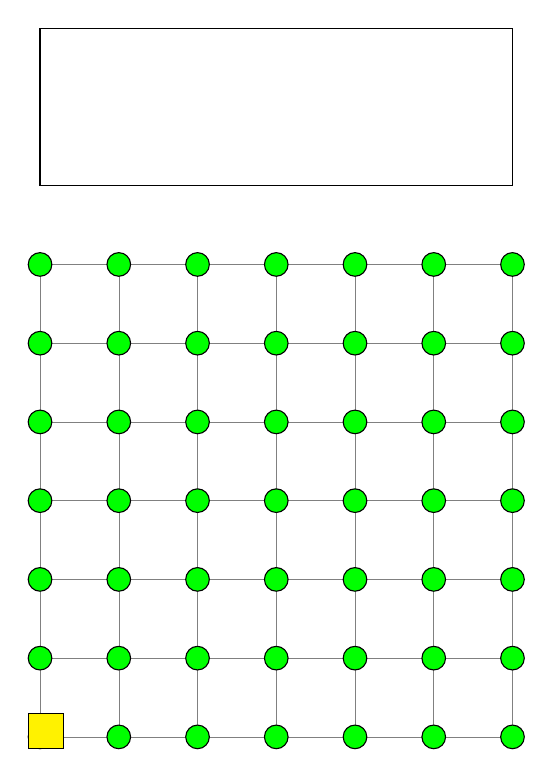
\begin{tikzpicture}[axis/.style={thin, black, ->, >=stealth'}]
	
		\def \nx {6}
		\def \ny {6}
		
	
		\draw (0, 7) rectangle (6,9);
		\draw[step=1cm,gray,very thin] (0,0) grid (\nx,\ny);
		\foreach \ix in {0,...,\nx}{
			\foreach \iy in {0,...,\ny}{
				\filldraw[fill=green] (\ix,\iy) circle (0.15);
			}
		}
		\filldraw[fill=yellow] (-0.15, -0.15) rectangle (0.3, 0.3);
%		\filldraw[fill=yellow] (0,0) circle (0.15);

	\end{tikzpicture}
	\caption{Caption}
	\label{fig:grid_of_nodes}
\end{figure}
	\input{figures/grid_of_nodes_B.tex}